\documentclass{article}
\usepackage[dblblindworkshop,nonatbib]{neurips_2026}
\workshoptitle{AIMO Interpretability Challenge}
\usepackage[utf8]{inputenc}
\usepackage[T1]{fontenc}
\usepackage{hyperref}
\usepackage{url}
\usepackage{booktabs}
\usepackage{amsmath}
\usepackage{graphicx}
\usepackage{microtype}
\input{glyphtounicode}
\pdfgentounicode=1
\usepackage{tikz}
\usetikzlibrary{positioning,arrows.meta}
\sloppy

\title{A Real Effect, an Unprovable Margin:\\Hidden-State Drift and the Limits of Evaluating\\Robustness Probes on Small Models}

\author{Anonymous Author(s)}

\begin{document}
\maketitle

\begin{abstract}
We predict whether a small language model's answer to a mathematics problem is robust to rewording, using no generation at all: we perturb the problem ourselves and measure how far the model's hidden states move. On the public Small Models test the probe scores 0.71 (10/14). A dedicated ablation shows that the hidden-state block carries the score: alone it keeps 0.71, and without it the score falls to 0.43. We then report what we could not establish. Eight follow-up white-box studies with fixed pass criteria failed, among them saliency, activation patching and aligned drift inside the reasoning trace. When we audited the evaluation itself, our own winning signal failed the same gates: problem length beats it on the only large labelled set, and 14 test cases cannot separate the ablations ($p=0.29$). Our main contribution is therefore methodological: without a positive control and a length-matched test, a robustness probe's pass or fail carries little information.
\end{abstract}

\section{Introduction}

The AIMO Interpretability Challenge asks for a prediction of whether a model stays correct when a problem is reworded \cite{aimo}. The direct route is to generate answers to perturbed problems, which is expensive. Our route uses seven prompt-only forward passes per case. The perturbation families are published, so we recreate the cheap ones and read the change in the model's internal state. The idea is that a model which has parsed the mathematics should encode a renamed problem almost identically.

We make three contributions. (1) A generation-free white-box probe, with a test-set ablation showing that its hidden-state signal drives the score (Section~\ref{sec:ablation}). (2) Negative results from studies whose criteria were committed before the data existed (Section~\ref{sec:negative}), including one causal measurement that does hold across all four models. (3) A positive-control audit showing why those negatives, and the leaderboard itself, are weaker evidence than they look, with concrete recommendations (Sections~\ref{sec:audit} and~\ref{sec:recs}).

\section{Submission}
\label{sec:method}

\textbf{Features.} For each case we build six deterministic perturbations of the problem: rename, numerals, typos, distract, rephrase and number jitter. Each prompt ends in the answer prefix \texttt{The final answer is \$\textbackslash boxed\{}, so the last position is the model committing to its answer. From one unbatched fp16 forward pass per prompt we read, at six depth fractions (0.25 to 1.0), the cosine and norm ratio of the last-token state against the original. This gives 72 hidden-state features. A further 15 come from the next-token distribution (KL, entropy, margin) and from flags for whether a perturbation applied. Hidden-state values are read at fp16 rounding scale, so prompts are never batched: batching changed the features (median $r=0.62$ between runs that differed only in batch composition).

\textbf{Training.} Only DeepSeek-R1-0528-Qwen3-8B has public labels, so a logistic classifier is fit on its 137 labelled MATH problems (36 robust), selecting feature count and regularisation by inner cross-validation. Nested CV estimates balanced accuracy at 0.60 and AUC at 0.67.

\textbf{Transfer without labels.} One artifact per checkpoint standardises each feature with that model's own statistics over a shared problem set. The threshold is that model's median margin over 173 unlabelled AIME/AMC problems (v2b). This assumes balanced hidden labels, which we inferred from the all-False and always-True submissions both scoring 0.50.

\textbf{Cost.} A full 14-case run across four models took about 83 s on the evaluation machine, against the 4200 s case limit. Figure~\ref{fig:pipeline} summarises the pipeline. Code, artifacts and bundles are in the repository \cite{repo}, with the submission in \texttt{submission/} and the follow-up studies in \texttt{self-perturb/}; Appendix~\ref{app:repro} lists what is needed to reproduce the scores.

\begin{figure}[t]
\centering
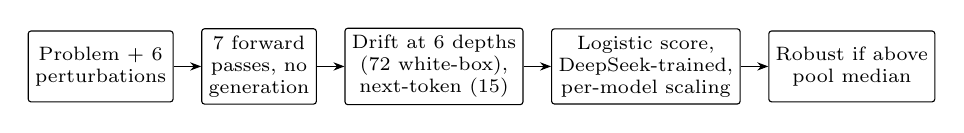
\begin{tikzpicture}[font=\scriptsize, node distance=3mm and 3.5mm,
  box/.style={draw, rounded corners=1pt, align=center, inner sep=2.5pt, minimum height=9mm},
  arr/.style={-{Stealth[length=1.4mm]}}]
\node[box] (p) {Problem $+$ 6\\perturbations};
\node[box, right=of p] (f) {7 forward\\passes, no\\generation};
\node[box, right=of f] (d) {Drift at 6 depths\\(72 white-box),\\next-token (15)};
\node[box, right=of d] (c) {Logistic score,\\DeepSeek-trained,\\per-model scaling};
\node[box, right=of c] (t) {Robust if above\\pool median};
\draw[arr] (p) -- (f); \draw[arr] (f) -- (d); \draw[arr] (d) -- (c); \draw[arr] (c) -- (t);
\end{tikzpicture}
\caption{The submitted probe. No answer is generated; 173 unlabelled pool problems set each model's threshold.}
\label{fig:pipeline}
\end{figure}

\section{White-box ablation}
\label{sec:ablation}

We rebuilt the submission twice. Each time the dropped block was mean-ablated (coefficients set to zero) and thresholds were reset at the pool median, so neither variant gained from seeing test data.

\begin{table}[h]
\centering
\caption{Ablation on the public test (14 cases). Coverage 1.0 and no invalid predictions throughout.}
\label{tab:ablation}
\begin{tabular}{lccc}
\toprule
Submission & Codabench ID & Accuracy & Correct \\
\midrule
Full v2b & 1014195 & 0.71 & 10/14 \\
Hidden-state block only & 1026158 & 0.71 & 10/14 \\
Without hidden-state block & 1019496 & 0.43 & 6/14 \\
\bottomrule
\end{tabular}
\end{table}

The white-box block keeps the whole score, and the remainder falls below chance. The effect is large at this resolution, four net cases. It is not statistically established: the two ablations disagree on 8 of 14 cases, split 6 to 2 in favour of the white-box signal (exact McNemar, two-sided $p=0.29$), and 10/14 itself occurs by chance with probability 0.09, before allowing for this being our best of many submissions. Offline nested CV on the labelled set agrees in direction: the hidden block reaches AUC 0.66 against 0.61 for the logit block and 0.56 for shuffled rows. Problem length alone, however, reaches 0.74 (Section~\ref{sec:audit}).

\begin{figure}[t]
\centering
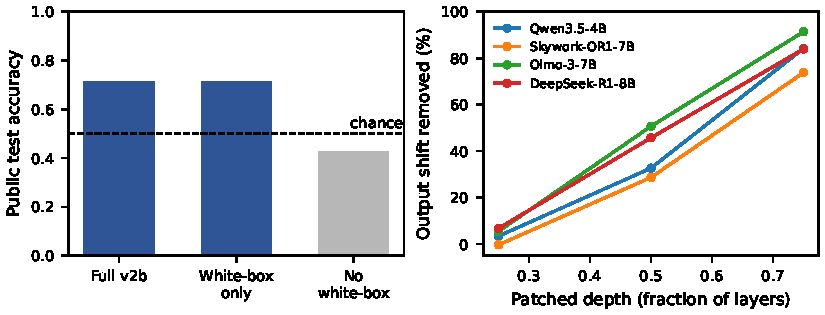
\includegraphics[width=\linewidth]{figure1.pdf}
\caption{Left: ablation on the public test. Right: share of the perturbation's output shift removed by restoring the original answer-position state at one depth (ratio of medians over 161 problems, five perturbations).}
\label{fig:main}
\end{figure}

\section{What makes this hard}

The label mechanism explains much of the difficulty. In the public tables, 80 of the 101 non-robust DeepSeek labels are caused by the \emph{domain} perturbation, which recasts the problem as a real-world story. Of 276 harmful domain variants, 88\% lack a number present in the original, and accuracy on those is 0.009 against 0.365 otherwise. So many non-robust labels may record lost information rather than a fragile model. Robust problems are also longer (27.9 words against 16.8), so short problems are non-robust for a reason unrelated to the model's internals, and any feature that tracks length inherits an apparent signal.

\section{Negative results}
\label{sec:negative}

Each study below followed one path: name what is failing, pick a method that addresses it, define a small sample, and commit the pass criteria before the run. Most were run on 2$\times$T4 in under an hour. train-main-v2 has only 22 labelled problems, and the self-domain set is the 137 labelled DeepSeek MATH problems.

\begin{table}[h]
\centering
\small
\caption{Follow-up studies. AUC is for predicting non-robust, with fixed sign unless noted. All failed.}
\label{tab:negative}
\begin{tabular}{p{0.26\linewidth}p{0.66\linewidth}}
\toprule
Study & Outcome \\
\midrule
T-019, v6: difficulty direction in question-only state & AUC 0.80 on train-main-v2, then 0.50 on the public test (Codabench 1018269, 1018354), including with a label-free pool-centred cut. \\
T-020: self-labelling & 26 labels in 4 h, $\kappa=-0.18$ against official labels. Not a usable substitute. \\
T-021: drift to a self-written domain rewrite & Adding white-box features lowered balanced accuracy from 0.67 to 0.58. \\
T-022: answer-recall contrast & Models recall only 3--12 of 173 pool problems immediately. No contrast. Fallback direction AUC 0.63, null $p=0.23$. \\
T-023: gradient$\times$input on prose vs.\ mathematics & AUC 0.36 on train-main-v2. Self-domain 0.69 ($p<0.001$), yet length alone gives 0.74. Saliency was NaN for Qwen3.5-4B. \\
T-024: activation patching at the answer position & Hook verified (identity KL 0), but AUC 0.39 and 0.54. Mechanism finding below. \\
T-025: drift along a replayed reasoning trace & Teacher forcing gives exact alignment (identity drift $3\times10^{-7}$), but AUC 0.30 and 0.59. \\
T-027: out-of-distribution arithmetic set & Failed its pilot gate: 95--100\% of answers exceeded the 1024-token cap, so no labels. The set was not tested. \\
\bottomrule
\end{tabular}
\end{table}

\textbf{One result that holds.} Activation patching \cite{pathpatching} replaces the answer-position state of a perturbed run with the original's at one layer. Patching at depth 0.25 removes 0--7\% of the output shift, at depth 0.5 removes 29--51\%, and at depth 0.75 removes 74--91\% (Figure~\ref{fig:main}, right). The pattern is the same on all four models: the perturbation's effect reaches the answer position between mid and late depth. This route did not predict the label, so it describes how perturbations travel, not which problems are robust.

\section{Auditing the gates}
\label{sec:audit}

After T-025 we scored v2's own drift with the same tests, as a positive control. It failed. On the self-domain set, unfitted mean drift scores AUC 0.54 ($p=0.28$) and the fitted hidden block 0.66, while length scores 0.74. A gate that rejects the signal behind our best score cannot be taken as evidence against other signals. One gate also compared with length in one direction only, which hid that short problems are the non-robust ones and made T-023's self-domain result look like a pass.

\begin{table}[h]
\centering
\small
\caption{The audit on the 137 self-domain problems (T-023: 132 scored). Stratified AUC compares only problems in the same length quartile, with $p$ from permutation inside quartiles.}
\label{tab:audit}
\begin{tabular}{lccc}
\toprule
Score & AUC & Stratified AUC & $p$ \\
\midrule
Problem length (short = non-robust) & 0.74 & --- & --- \\
v2 hidden block, fitted out-of-fold (control) & 0.66 & 0.58 & 0.09 \\
T-023 saliency & 0.69 & 0.65 & 0.008 \\
T-024 patching recovery & 0.54 & 0.55 & 0.24 \\
T-025 reasoning drift & 0.59 & 0.53 & 0.34 \\
\bottomrule
\end{tabular}
\end{table}

Next we fixed a length-matched gate before scoring. It computes AUC only between problems in the same length quartile, and its null permutes labels within quartiles. We would trust the gate only if the fitted v2 block passed it (AUC $\ge 0.60$, $p<0.05$). The block scored 0.58 ($p=0.09$), so the gate gives no verdict on the other signals. Their scores were 0.55 (T-024), 0.53 (T-025) and 0.65 (T-023, $p=0.008$). T-023 is the only signal that remains after matching length. But we chose that analysis after seeing the data, and on the 26 T-020 labels T-023 scored 0.35. Those labels disagree with the official ones, so that check is also weak.

The results seem to conflict: a strong ablation on the test set, and a weak signal on the labelled set. Two explanations remain open and we cannot separate them. The drift signal may be real on competition problems, which are about three times longer than the MATH training problems, and absent on short ones. Or the 0.71 may be partly chance. A test of 14 cases cannot decide.

\section{Recommendations}
\label{sec:recs}

For anyone evaluating robustness probes: (1) score a known signal as a positive control before trusting any gate, and treat a failed control as no verdict; (2) compare with length in both directions and prefer a length-matched test, because of how the labels arise; (3) report exact tests on discordant cases, since 14 cases give a one-case resolution of 7 points; (4) keep the sign and threshold fixed in advance, as a thresholded ranking from a 72\%-robust training set became near-constant on a balanced test; (5) for organisers, labels for more than one small model, and separating information-losing domain variants from the rest, would make these questions answerable.

\section*{Limitations}

The public test has 14 cases, so every test comparison here has very low power. Labels for hidden test cases were partly inferred from public scores: we learned that labels are balanced and something about a few individual cases, and we stopped using such inference once we recognised the overfitting risk. v2b's thresholds depend on the inferred balance. An earlier diagnostic submission (1014184) logged per-case margins during evaluation. We used it to compare per-case predictions, and we disclose it as evaluation-time logging. The final probes contain no test-derived values. AIME/AMC pool problems were used unlabelled, for thresholds and difficulty metadata. The classifier is trained on one model and transferred to three others with no labels, so we cannot measure accuracy per model. Our offline positive control uses short MATH problems, unlike the test. T-027 was not a fair test of the out-of-distribution idea, because our token cap was too low. Exploratory analyses are marked as such; T-026 returned no verdict by its own rule.

\section*{AI usage statement}

This work was done by one human author with AI assistance. Claude Code (Anthropic) wrote most of the code in the repository, ran the experiments on Kaggle under the author's direction, analysed results and drafted this report. Grok (xAI) executed some compute tasks. The author set the research direction, made all Codabench submissions, and reviewed the final text. Pass criteria were committed before each run; the git history records the order.

\begin{thebibliography}{9}
\bibitem{aimo} AIMO Interpretability Challenge. \url{https://aimo-interp.github.io/}, 2026.
\bibitem{repo} Anonymous. Self-perturbation probes for the AIMO Interpretability Challenge. Anonymised repository: \url{https://anonymous.4open.science/r/aimo-interp-log}, 2026.
\bibitem{pathpatching} N. Goldowsky-Dill, C. MacLeod, L. Sato, A. Arora. Localizing model behavior with path patching. arXiv:2304.05969, 2023.
\bibitem{saliency} A. Shrikumar, P. Greenside, A. Kundaje. Learning important features through propagating activation differences. In \emph{ICML}, 2017.
\end{thebibliography}

\appendix
\section{Reproduction}
\label{app:repro}

\textbf{Layout.} Submission code and bundles are in \texttt{submission/}; the paths under Bundles, Training data and the first Pipeline sentence are relative to it. Follow-up studies are in \texttt{self-perturb/}, and this report is in \texttt{report/}.

\textbf{Bundles.} Under \texttt{results/submissions/}, with the prefix \texttt{solution-v2b-} and the suffix \texttt{-small.zip}: \texttt{poolthr} (1014195), \texttt{ablate-wbonly} (1026158), \texttt{ablate-nowb} (1019496). Other IDs cited: 1014184, 1018269, 1018354.

\textbf{Training data.} The organisers' public labelled DeepSeek MATH problems; the 173 AIME/AMC pool problems in \texttt{data/pool\_unlabelled.parquet}. No evaluation data.

\textbf{Environment.} torch 2.11.0+cu128 (training features on 2$\times$T4), transformers 5.13.0, fp16, unbatched.

\textbf{Pipeline.} \texttt{scripts/dump\_features.py}, \texttt{scripts/evaluate.py}, \texttt{scripts/calibrate\_per\_model.py}, \texttt{scripts/build\_bundle.py}. Ablations: \texttt{scripts/ablate\_whitebox.py}. The two ablation bundles were made from the v2b bundle by setting the dropped block's coefficients to zero and re-setting each threshold at the pool median. Follow-up studies: \texttt{self-perturb/scripts/} (\texttt{dump\_*}, \texttt{eval\_*}) with outputs in \texttt{self-perturb/results/grok/T-0xx/}. Pass criteria are in each \texttt{eval\_*} docstring, committed before its run.

\end{document}
